\documentclass[11pt,fleqn,twoside]{article}
\usepackage{makeidx}
\makeindex
\usepackage{palatino} %or {times} etc
\usepackage{plain} %bibliography style 
\usepackage{amsmath} %math fonts - just in case
\usepackage{amsfonts} %math fonts
\usepackage{amssymb} %math fonts
\usepackage{lastpage} %for footer page numbers
\usepackage{fancyhdr} %header and footer package
\usepackage{mmpv2} 
\usepackage{url}

\usepackage{graphicx}
\usepackage{algpseudocode}
\usepackage{multirow}
\usepackage{listings}
\usepackage{float}

% the following packages are used for citations - You only need to include one. 
%
% Use the cite package if you are using the numeric style (e.g. IEEEannot). 
% Use the natbib package if you are using the author-date style (e.g. authordate2annot). 
% Only use one of these and comment out the other one. 
\usepackage{cite}
%\usepackage{natbib}

\begin{document}

\name{Alexander D. Brown}
\userid{adb9}
\projecttitle{Kyffin Williams: Digital Analysis of Paintings}
\projecttitlememoir{Kyffin Williams: Digital Analysis of Paintings} %same as the project title or abridged version for page header
\reporttitle{Progress Report}
\version{0.1}
\docstatus{Draft}
\modulecode{CS39440}
\supervisor{Hannah M. Dee} % e.g. Neil Taylor
\supervisorid{hmd1}
\wordcount{?} %TODO

%optional - comment out next line to use current date for the document
%\documentdate{26th October 2011} 
\mmp

\setcounter{tocdepth}{3} %set required number of level in table of contents
\tableofcontents
\listoffigures
\listoftables

\newpage

%==============================================================================
\section{Project Summary}
%==============================================================================
Sir John ``Kyffin'' Williams was a landscape painter from Wales whose work was predominantly based 
in Wales and Patagonia. His work, with associated metadata collected by Gareth Lloyd Roderick and 
the National Library of Wales, allows for some interesting analysis; particularly that of temporal 
or geological data for a given painting.

Temporal analysis will be the focus of this project as it allows for a diverse range of techniques;
from statistical analysis of RGB values of the paintings to looking at the length and style of 
paintbrush strokes. 

Whilst it would be nice to be able to predict the age of a painting with no known year, it is far
more interesting to try to guess the year of paintings where the date is known. This allows for
cross-validation of the techniques employed to guess the year. This project will use leave-one-out
cross-validation for simplicity as the data set is small enough to allow this computationally 
expensive technique.

%==============================================================================
\section{Current Progress}
%==============================================================================

\subsection{Library and Language Research}
The first step in the project was to research into the numerous image processing/computer vision
libraries available for use with the aim to find the most suitable library to use constantly for 
the rest of the project. Because of this the library had to be easy to install and use, as well as
having all the necessary features which would be used in this project.

The choice of library would also have a knock-on affect on the choice of language this project 
would be written in. To this end I downloaded each of the libraries in turn, created a simple 
application to perform blur on a simple image to test their use and documentation. From this I
gained a good insight into how easy that library would be to perform more complex tasks and how
confident I felt with the language(s) the library had bindings for.

Table~\ref{tab:libraries-overview} shows an overview of all the libraries I have currently 
considered and experimented with.

\begin{table}[h]
\begin{tabular}{| c | c | c | c | c | c | c |}
								  \hline
\multirow{2}{*}{\textbf{Library}}	& \multicolumn{4}{|c|}{\textbf{Platform}}			& \multirow{2}{*}{\textbf{Language(s)}}	& \textbf{Example}	\\\cline{2-5}
					&  Windows	& Mac 		& Linux 	& Android	&					&			\\\hline
OpenCV					& \checkmark	& \checkmark	& \checkmark	& \checkmark	& C, C++, Python			& Figure~\ref{fig:opencv}\\\hline
FIJI					& \checkmark	& \checkmark	& \checkmark	& 		& Java					& Figure~\ref{fig:fiji}	\\\hline
IVT					& \checkmark	& \checkmark	& \checkmark	& 		& C++					& Figure~\ref{fig:ivt}	\\\hline
VXL					& \checkmark	& \checkmark	& \checkmark	& 		& C++					& Figure~\ref{fig:vxt}	\\\hline
\end{tabular}
\caption{Comparison of image processing/computer vision libraries.}
\label{tab:libraries-overview}
\end{table}

Of these libraries OpenCV was the easiest to work with. OpenCV also boasts a wide range of 
features, all of which are well documented. FIJI provided a lot of high-level functionality, but
for use as a library it quickly became unwieldy and was difficult to find the correct classes just 
for the simple task of blurring an image. On a side note, I only managed to get the blurring 
outputting a greyscale image in the short period of time I spent using FIJI.

IVT was somewhat similar to FIJI in that it had a good range of high-level features, but was less
impressive as a library. Despite following the example code I struggled to compile my own example
and eventually gave up trying to get a working binary due to time constraints.

%TODO Actually use VXL and then write about it.

Having decided to go with OpenCV I was then faced with a choice of languages. OpenCV runs natively
with C++ and has bindings for Python. Of these two languages I am slightly more familiar with C++. 
I am also used to the syntax from programming Java continually for three years. 

However, I wanted to take a rapid prototyping approach with this project; constantly adding new 
modules each week to build up a better and better system. C++ seemed too heavyweight for this 
approach, whilst Python seemed designed for it.

Another consideration I had was that the results of any analysis could take any form at all, from
an array of numbers to a complex data structure returned by OpenCV. Trying to work around this with
a statically typed language such as C++ could end up being difficult, especially when trying to 
keep a object-orientated approach.

With a dynamically typed language such as Python it's a lot easier to pass these sorts of objects
so long as the functions you pass to are expecting the right sort of object. There may be some 
parts of the project which I might consider writing in C++ after prototyping in Python. An example
of this would be if I wrote an algorithm which located strokes across the painting, as it may be
used in other projects, not just my own.


\begin{figure}[p]
\begin{lstlisting}[language=Python]
import cv

im = cv.LoadImageM("tux.png")
blur = cv.CreateMat(im.rows, im.cols, im.type)
cv.Smooth(im, blur, cv.CV_BLUR, 9)
cv.SaveImage("tux_blurred_opencv.png", blur)
\end{lstlisting}
\caption{Using OpenCV to blur an image}
\label{fig:opencv}
\end{figure}

\begin{figure}[p]
\begin{lstlisting}[language=Java]
package fiji;

import ij.IJ;
import ij.io.FileSaver;
import imagescience.feature.Smoother;
import imagescience.image.ColorImage;
import imagescience.image.Image;

public final class Blur {
	public static final String IMG_PATH = "tux.png";
	public static final String OUTPUT_PATH = "tux_fiji.png";

	public static void main(String[] args) {
		final Image image = new ColorImage(IJ.openImage(IMG_PATH));
		final Smoother s = new Smoother();
		final Image blurred = s.gauss(image, 9f);
		final FileSaver fs = new FileSaver(blurred.imageplus());
		fs.saveAsPng(OUTPUT_PATH);
	}
}
\end{lstlisting}
\caption{Using FIJI to blur an image}
\label{fig:fiji}
\end{figure}

\begin{figure}[p]
\begin{lstlisting}[language=C++]
#include <stdio.h>
#include "Image/ByteImage.h"
#include "Image/ImageProcessor.h"

int main(int argc, char **argv) {
	if(argc != 2) {
		fprintf(stderr, "Usage: ivt input output\n");
		return 1;
	}

	CByteImage in;
	CByteImage out;

	if(!in.LoadFromFile(argv[0])) {
		fprintf(stderr, "Unable to load file %s\n", argv[0]);
		return 2;
	}

	out = CByteImage(in);
	ImageProcessor::GaussianSmooth(&in, &out, 1.0f, 3);
	if(!out.SaveToFile(argv[1])) {
		fprintf(stderr, "Unable to save to file %s\n", argv[1]);
	}
}
\end{lstlisting}
\caption{Using IVT to blur an image}
\label{fig:ivt}
\end{figure}

\begin{figure}[p]
\caption{Using VXT to blur an image}
\label{fig:vxt}
\end{figure}

\subsection{Other Tools}
Having used git for several personal projects I was keen to continue using it for my version 
control. GitHub was a convenient hosting company to go with as they provide students with free 
private repositories and have very high uptime. It also means I am able to easily work on any 
system without difficulty but with the assurance of security. This is preferable to hosting my own
repositories and running the risk of losing a lot of work.

\subsection{Design}
\begin{figure}[H]
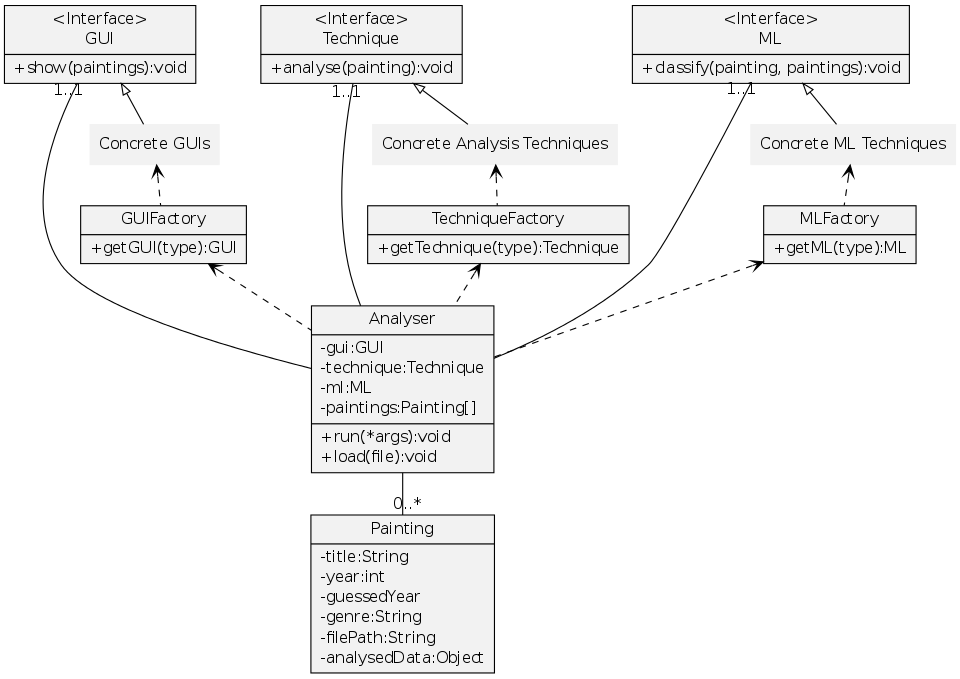
\includegraphics[scale=0.5]{img/design.png}
\caption{Initial Design}
\label{fig:init-class}
\end{figure}

An initial UML class diagram is depicted by figure~\ref{fig:init-class}. This design will allow 
additional techniques, both analysis and machine learning based, to be added easily. Command line
arguments, or later a GUI front-end, will be used to specify which techniques should be used.

The GUI elements depicted are used for visualising the analysed data or results of the machine
learning algorithms. An example of this is a graphical representation of the colour space averages
(see figure~\ref{fig:mean-hsv-by-year}).

\subsection{Colour Space Statistical Analysis}
With the design solidified, I begun to work on the statistical analysis of digital images. The 
easiest of these techniques is to read the image pixel by pixel, taking the various intensities at
that pixel, then averaging them out over the whole image.

The most common colour space used is RGB (Red, Green, Blue), where each pixel holds three different
intensities, one for each colour with a value of 0 to 255.

Using this analysis I plotted a graph of all paintings with a known year against the different 
intensities (see figure~\ref{fig:mean-rgb-by-year}). As can be seen from this graph, the RGB values
tend to fluctuate without much correlation between year.

\begin{figure}[p]
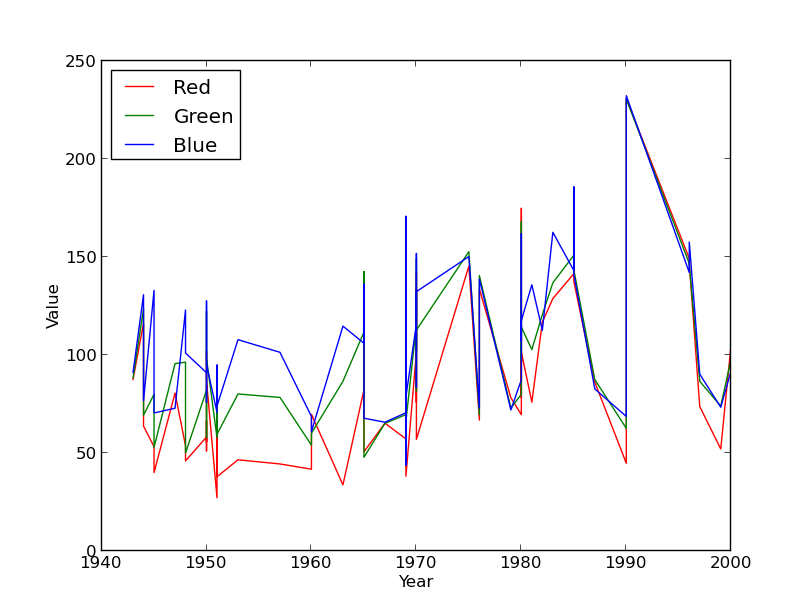
\includegraphics[scale=0.5]{img/kyffin-rgp-avg.png}
\caption{Mean RGB intensities by year.}
\label{fig:mean-rgb-by-year}
\end{figure}

Another popular colour space used in image processing is HSV (Hue, Saturation, Value) as it shows
variations in colour, saturation and brightness separately (unlike RGB where all three values are
affected by changes in brightness). It was a simple matter of changing the existing code for RGB
so that it would analyse HSV values instead.

I also decided it would be an improvement to average all values in the same year together to help
show changes as time goes on (see figure~\ref{fig:mean-hsv-by-year}).

\begin{figure}[p]
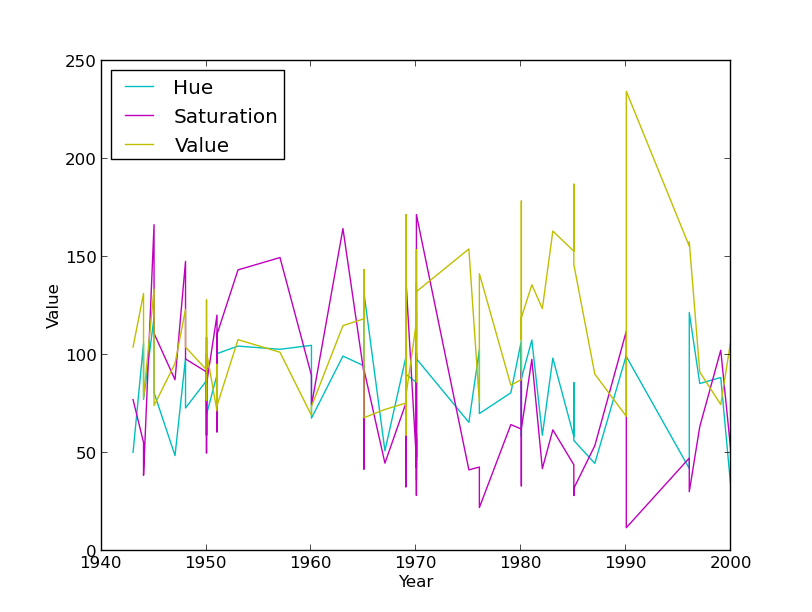
\includegraphics[scale=0.5]{img/hsv-legend-12-11-01.png}
\caption{Mean HSV intensities by year.}
\label{fig:mean-hsv-by-year}
\end{figure}


\subsection{Histogram Analysis}
With colour-space analysis complete, the next sensible step was to start generating colour 
histograms from Kyffin Williams paintings.

A histogram is a nice way of displaying the distribution of colour in a given image and is 
therefore a more useful representation of a painting than colour-space averages.

As with before, histograms can be taken from different colour spaces, currently only the program
can only generate RGB histograms, but it is trivial to include HSV histograms too.

\subsection{Nearest Neighbour Classification}
Having finished the analysis techniques, then next part was to create a simple classification 
algorithm. The simplest of which is 1-Nearest Neighbour, that is; take the ``Nearest'' training
example to the example to be classified and classify the year of this example with the year of the
nearest example (see figure~\ref{fig:1-nn}).

This simple algorithm can be expanded to be a K-Nearest Neighbour algorithm without too much effort
(see figure~\ref{fig:k-nn}).

\begin{figure}[h]
\begin{algorithmic}
\State $bestDistance \gets \infty$
\For{$x = 1 \to X$}
	\If{$distance(a, x) < bestDistance$}
		\State $bestDistance \gets distance(a, x)$
	\EndIf
\EndFor
\end{algorithmic}

Where:\\
\(a\) is the example to classify.\\
\(X\) is the list of all training examples.
\caption{1-Nearest Neighbour}
\label{fig:1-nn}
\end{figure}

\begin{figure}[h]
\begin{algorithmic}
\State $kBest \gets []$
\For{$x = 1 \to X$}
	\State $cur \gets distance(a, x)$
	\For{$k = 1 \to K$}
		\If{$cur < kBest[k]$}
			\State $temp \gets kBest[k]$
			\State $kBest[k] \gets cur$
			\State $cur \gets temp$
		\EndIf
	\EndFor
\EndFor
\end{algorithmic}
Where:\\
$a$ is the example to classify.\\
$X$ is the list of all training examples.
$K$ is the number of nearest neighbours to check.
\caption{K-Nearest Neighbour}
\label{fig:k-nn}
\end{figure}


\subsection{Distance Measures}
Working out the ``Nearest'' example to a given painting requires some way of measuring distance
between the two.

One very simple way of doing this is Manhattan distance (figure~\ref{eq:manhattan}). This distance
measure can be improved further to euclidean distance (figure~\ref{eq:euclidean}) without too much
effort. There are numerous other methods of measuring the distance of points in space, including
those which focus on the distance between colour histograms.

\begin{figure}[h]
\[
d = \sum^X_{x=0}{|a_x - b_x|}
\]

\(X\): All dimensions present in both \(a\) and \(b\).\\
\(a\): The first point.\\
\(b\): The second point.

\caption{Manhattan Distance}
\label{eq:manhattan}
\end{figure}

\begin{figure}[h]
\[
d = \sqrt{\sum^X_{x=0}{(a_x - b_x)^2}}
\]

\(X\): All dimensions present in both \(a\) and \(b\).\\
\(a\): The first point.\\
\(b\): The second point.
\caption{Euclidean Distance}
\label{eq:euclidean}
\end{figure}


\subsection{Meetings with Gareth Lloyd Roderick}
At current I have had one meeting with both Lloyd and Hannah to discuss the current progress of 
the project and where we see the project progressing to. Lloyd was impressed by the current state
of the project and was looking forward to see where it was leading to.

We also discussed the potential of getting a paper published out of this project.

\subsection{Research into Stroke Analysis}
Stroke analysis is one of the main goals for this project. It is quite apparent from looking at 
Kyffin Williams' paintings that his brushstrokes change over time, his early work having lots of
smaller strokes over the canvas to large bold strokes in his later work.

The first paper I found relating to the analysis of brushstrokes involved moving a circular filter
across the whole painting to find the ridges of strokes, then to fill any unbroken areas. They then
shrunk these areas to a single pixel line and fitted a $n^{\text{th}}$ order polynomial to this
line\cite{Berezhnoy2005Authentic}. This method seems fairly simplistic, but could be an interesting
first step, but as it is more focused on authenticating paintings it may be of limited use.




%==============================================================================
\section{Planning}
%==============================================================================



%==============================================================================
\section*{Your Bibliography - REMOVE for final version}
%==============================================================================
%
%You need to include an annotated bibliography. This should list all relevant web pages, books, journals etc. that you have consulted in researching your project. Each reference should include an annotation. 

%The purpose of the section is to understand what sources you are looking at.  A correctly formatted list of items is sufficient. You might go further and make use of bibliographic tools, e.g. BibTeX in a LaTeX document, could be used to provide citations, for example \cite{NumericalRecipes} \cite{MarksPaper} \cite[99-101]{FailBlog} \cite{kittenpic_ref}.  The bibliographic tools are not a requirement, but you are welcome to use them.   

%You can remove the above {\em Your Bibliography} section heading because it will be added in by the renewcommand which is part of the bibliography. The correct annotated bibliography information is provided below. 
%
% End of comment out / remove the lines. They are only provided for instruction for this example template. 
%


\nocite{*} % include everything from the bibliography, irrespective of whether it has been referenced.

% the following line is included so that the bibliography is also shown in the table of contents. There is the possibility that this is added to the previous page for the bibliography. To address this, a newline is added so that it appears on the first page for the bibliography. 
\newpage
\addcontentsline{toc}{section}{Annotated Bibliography} 

%
% example of including an annotated bibliography. The current style is an author date one. If you want to change, comment out the line and uncomment the subsequent line. You should also modify the packages included at the top (see the notes earlier in the file) and then trash your aux files and re-run. 
%\bibliographystyle{authordate2annot}
\bibliographystyle{IEEEannot}
\renewcommand{\refname}{Annotated Bibliography}  % if you put text into the final {} on this line, you will get an extra title, e.g. References. This isn't necessary for the outline project specification. 
\bibliography{mmp} % References file


\end{document}
